%_______________________________________________________________________________
% main.tex

\input{preamble12.tex}
\hypersetup{%
    pdfauthor={Mike Pierce}%
   ,pdftitle={Pop Quiz | Math 113}%
   ,pdfkeywords={Pierce,CMU,Colorado,College Algebra,113}%
   ,pageanchor=false%
}
\geometry{
    margin=1in%
   ,left=0.75in%
   ,right=0.75in%
}
\usepackage{fourier}
\usepackage[default]{comicneue}
\input{accessible-colors.tex}
\input{newcommand.tex}
\input{newenvironment.tex}
\pagenumbering{gobble}
\usepackage{pagegrid}
\pagegridsetup{
    step=0.5in
    ,firstcolor=blue
    ,secondcolor=orange
    ,foreground=true
    ,disable
}


\begin{document}

\begin{center}
    {\Huge{Pop Quiz}}
    \\ Math 113-001/6 College Algebra
    \\ Colorado Mesa University Fall 2022
\end{center}

\vspace{2em}
\textsc{Name}: \enspace \hrulefill
\vspace{1em}

\begin{enumerate}

    \item 
        What are the coordinates of the vertex
        and of the two \(x\)-intercepts of the parabola
        that is the graph of \(f(x) = -3-4x-x^2\)?
        % vertex (-2, 1)
        % roots at -1 and -3
        \vfill\null
        \vfill\null

    \item 
        According to the US Census Bureau,
        the population of the United States
        can be modelled by the function \(p(t) = 165.6t^{1.345}\)
        where \(p(t)\) is measured in thousands of people
        and \(t\) is measured in years since 1800.
        \begin{enumerate}
            \item
                According to this model, what was the population
                of the US in the year 1942?
                \vfill\null
            \item 
                Independent of this model, 
                the US Census Bureau estimates 
                that the \emph{current} US population 
                is \(332,403,650\) people.
                How does this estimate compare to the 
                current US population that their model predicts?
                \vfill\null
                \vfill\null
        \end{enumerate}

        \newpage

    \item 
        % piecewise-defined functions
        Let \(g\) be the function defined piecewise as 
        \begin{equation*}
            g(x) = \begin{cases} 
                -1 &\text{ if } x < -3
                \\ x + 3 &\text{ if } -3 \leq x < 1
                \\-x^2+5 &\text{ if } 1 \leq x
            \end{cases}
        \end{equation*}
        \begin{enumerate}
            \item 
                Accurately sketch the graph \(y = g(x)\) 
                on the axis below,
                and on your sketch label all of the following
                points with their coordinates:
                \begin{itemize}\setlength\itemsep{-1em}
                    \item the \(y\)-intercept and \emph{all} \(x\)-intercepts
                    \item the points \((-4,g(-4))\), \((5,g(5))\), \(-3, g(-3)\), and \(1, g(1)\).
                    \item the point where \(g\) attains its maximum value
                \end{itemize}
            \begin{figure}[h]
                \centering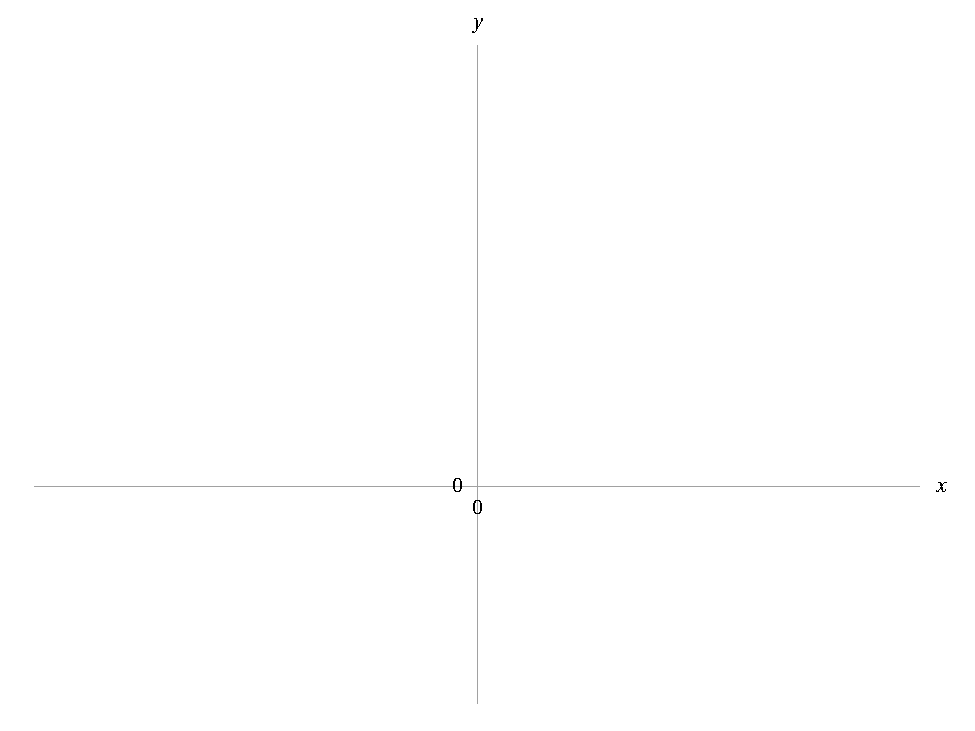
\includegraphics[width=0.92\textwidth]{figures/blank/main.pdf}
            \end{figure}
            \item (\textsc{Challenge})
                You'll notice that the graph of \(g\) 
                is not a ``continuous'' curve:
                the pieces of the graph of \(g\)
                don't line up with each other at \(x=-3\).
                How could you change the formula
                for the ``middle'' piece of \(g\) where
                \(-3 \leq x < 1\) in such a way that 
                the three pieces of the graph would connect?
                % \frac{5}{4}x + \frac{11}{4}
        \end{enumerate}

\end{enumerate}

\end{document}

